\section{Einleitung} % (fold)
\label{sec:einleitung}

Der Reinst-Germanium-Detektor ist ein Messinstrument in der $\gamma$-Spektroskopie.
Der Detektor besitzt im Vergleich zu anderen Detektoren ein hohes Energieauflösungsvermögen und in diesem Versuch werden die $\gamma$-Spektren verschiedener Proben untersucht.

\section{Theorie} % (fold)
\label{sec:theorie}

\subsection{Wechselwirkung von $\gamma$-Strahlung mit Materie} % (fold)
\label{sub:wechselwirkung_von_gamma_strahlung_mit_materie}

Tritt ein $\gamma$-Quant mit Materie in Wechselwirkung, sind für die $\gamma$-Spektroskopie besonders der Photoeffekt, der Compton-Effekt und die Paarbildung von Interesse.
Diese Effekte führen zu einem vom Wirkungsquerschnitt $\sigma$ abhängigen Intensitätsverlust des $\gamma$-Strahls.
Die Intensität kann mithilfe der Gleichung

\begin{equation}
	N(D) = N_\text{0} \left(1-\exp\left(- n \sigma D\right)\right)
\end{equation}

beschrieben werden.
Dabei ist $D$ die Absorberschichtdicke, $N_\text{0}$ die ursprüngliche Strahlintensität und $n$ die Teilchendichte des Absorbers.\\

Die mittlere Reichweite $\bar{x}$ der $\gamma$-Quanten ist durch den reziproken Wert des Extinktionskoeffizenten gegeben.
Unter der Annahme von isolierten Elektronen der Absorberatome ist dieser durch

\begin{equation}
	\mu = n \sigma = \frac{z N_\text{L} \rho}{A} \sigma
\end{equation}

gegeben.
$A$ entspricht dem Atomgewicht, $\rho$ der Dichte, $z$ der Kernladungszahl und $N_\text{L}$ der Loschmidtschen Zahl.\\

Beim Photoeffekt muss die Energie des $\gamma$-Quants $E_\gamma$ größer sein als die Bindungsenergie $E_\text{B}$ der Elektronen.
Dabei gibt der $\gamma$-Quant seine gesamte Energie an das Elektron ab, sodass dieses die Energiedifferenz als kinetische Energie erhält.
Die entstandenen Elektronenlöcher werden unter Aussendung charakteristischer Röntgenstrahler von einem Elektron einer höheren Schale aufgefüllt.
Der Wirkungsquerschnitt des Photoeffekts ist durch

\begin{equation}
	\sigma_\text{ph} \propto z^\alpha E^\delta \label{photo_quer}
\end{equation}

gegeben mit 4 < $\alpha$ < 5 und $\delta \approx$ -3,5.\\

\begin{figure}
	\centering
	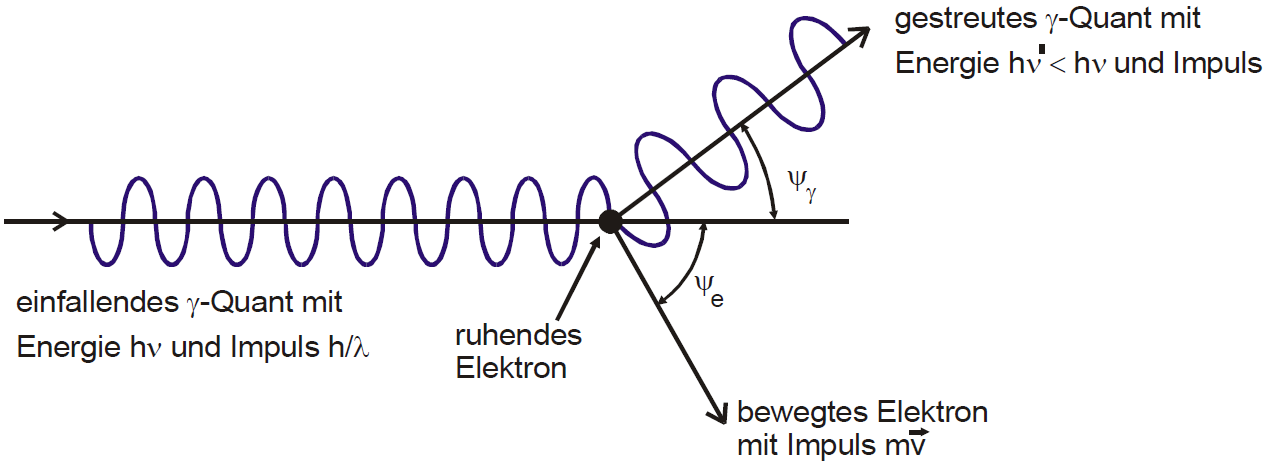
\includegraphics[width = 0.5\textwidth]{pic/compton.png}
	\caption{Schematische Darstellung der Compton-Streuung \cite{anleitung}.}
	\label{compton}
\end{figure}

Der Compton-Effekt kann als inelastische Streuung des $\gamma$-Quants an einem praktisch ruhenden Elektron verstanden werden.
Mit

\begin{equation}
	\epsilon = \frac{E_\gamma}{m_\text{0} c^2}
\end{equation}
ergibt sich nach Abbildung \ref{compton} für die Energie des gestoßenen Elektrons

\begin{equation}
	E_\text{el} = E_\gamma - E_{\gamma'} = E_\gamma \frac{\epsilon (1-\cos{\Psi_\gamma})}{1 + \epsilon (1-\cos{\Psi_\gamma})} . 
\end{equation}

Somit ist der maximale Energieübertrag durch 

\begin{equation}
	E_\text{el,max} = E_\gamma \frac{2\epsilon}{1+2\epsilon} < E_\gamma
\end{equation}

gegeben.
Somit ist der Compton-Effekt eine unerwünschte Erscheinung, da nur ein sich verändernder Bruchteil der $\gamma$-Energie detektiert wird.\\

\begin{figure}
	\centering
	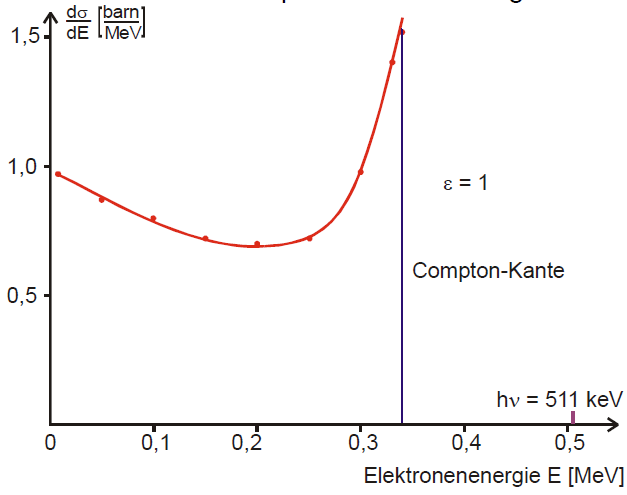
\includegraphics[width = 0.5\textwidth]{pic/compton2.png}
	\caption{Differentieller Wirkungsquerschnitt für die Compton Streuung bei $\epsilon = 1$ \cite{anleitung}.}
	\label{compton2}
\end{figure}
Bei kleinen Energien gilt für den Wirkungsquerschnitt 

\begin{equation}
	\sigma_\text{Co} = \frac{3}{4} \sigma_\text{Th} \left(1 - 2\epsilon + \frac{26}{5} \epsilon^2 + ...\right) .
\end{equation}

Für $\epsilon \rightarrow 0$ gilt

\begin{equation}
	\sigma_\text{Co} = \sigma_\text{Th} = \frac{8}{3} \pi \r_\text{el}^2 . 
\end{equation}

Da Detektoren nur die Elektronenenergie detektieren, ist die Energieverteilung der gestoßenen Elektronen wichtig.
Diese ist durch den differentiellen Wikrungsquerschnitt $\frac{\text{d}\sigma}{\text{d}E}$ gegeben.
In Abbildung \ref{compton2} ist eine beispielhafte Kurve dargestellt.
\FloatBarrier

